\documentclass[tikz, border=20pt]{standalone}
\usepackage{amsmath, amssymb}
\usetikzlibrary{calc, arrows.meta, positioning, decorations.pathreplacing, decorations.markings}

\begin{document}
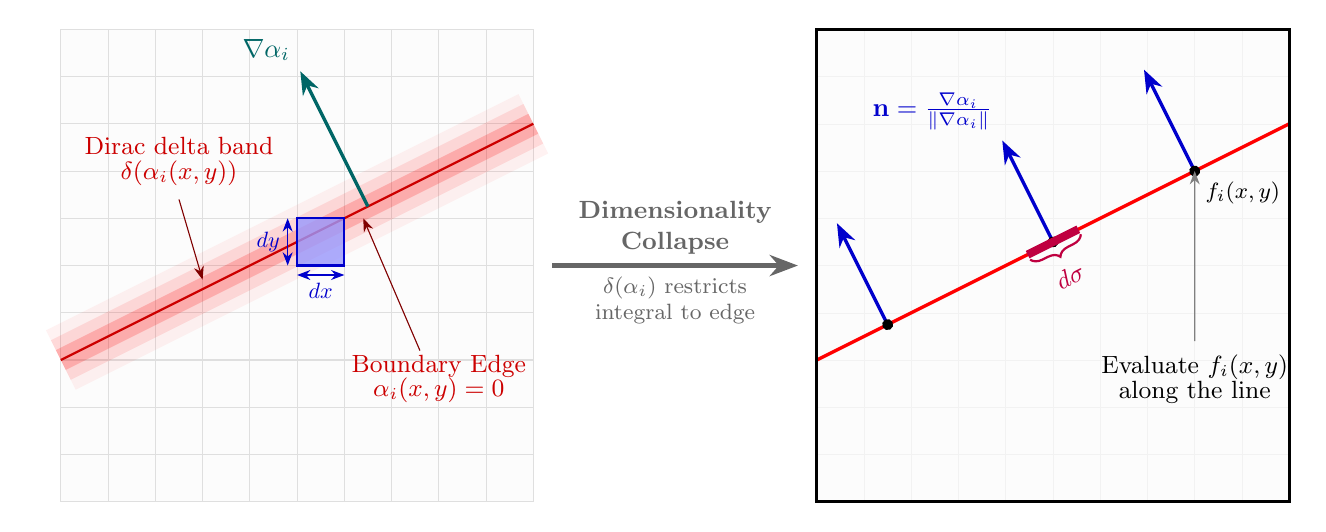
\begin{tikzpicture}[x=1.2cm, y=1.2cm, >=Stealth]

    % ==========================================
    % MACRO: The Straight Line Path
    % ==========================================
    % A straight line representing the triangle boundary edge \alpha_i(x,y) = 0
    \def\curvepath{(0, 1.5) -- (5, 4)}

    % ==========================================
    % PANEL 1: 2D Area Integral View
    % ==========================================
    \begin{scope}[shift={(0,0)}]
        % Background and Grid
        \fill[gray!2] (0,0) rectangle (5,5);
        \draw[step=0.5, gray!25, thin] (0,0) grid (5,5);

        % The Dirac Delta "Glow" Distribution (concentrating area to the line)
        \draw[red, line width=24pt, opacity=0.05] \curvepath;
        \draw[red, line width=16pt, opacity=0.10] \curvepath;
        \draw[red, line width=8pt, opacity=0.20]  \curvepath;
        
        % The actual line boundary
        \draw[red!80!black, thick, postaction={
            decorate,
            decoration={
                markings,
                % Unnormalized Gradient Vector \nabla \alpha
                mark=at position 0.65 with {
                    \draw[->, teal!80!black, very thick] (0,0) -- (0, 1.6) 
                        node[above left, scale=0.95] {$\nabla\alpha_i$};
                }
            }
        }] \curvepath;

        % Annotations for Dirac Delta and Edge
        \node[red!80!black, font=\small, align=center] at (1.25, 3.6) {Dirac delta band\\[-2pt]$\delta(\alpha_i(x,y))$};
        \draw[->, red!50!black, thin] (1.25, 3.2) -- (1.5, 2.35);

        \node[red!80!black, font=\small, align=center] at (4, 1.3) {Boundary Edge\\[-2pt]$\alpha_i(x,y) = 0$};
        \draw[->, red!50!black, thin] (3.8, 1.6) -- (3.2, 3.0);

        % The Area Element dx dy (Placed so the line cleanly slices it)
        \fill[blue!40, fill opacity=0.8] (2.5, 2.5) rectangle (3.0, 3.0);
        \draw[blue!80!black, thick] (2.5, 2.5) rectangle (3.0, 3.0);
        
        \draw[<->, blue!80!black, thin] (2.5, 2.4) -- (3.0, 2.4) node[midway, below, scale=0.8] {$dx$};
        \draw[<->, blue!80!black, thin] (2.4, 2.5) -- (2.4, 3.0) node[midway, left, scale=0.8] {$dy$};

        % % Pixel/Domain Border
        % \draw[very thick, black] (0,0) rectangle (5,5);

        % % Equation Text
        % \node[align=center, yshift=-2.2cm] at (2.5, 0) {
        %     \textbf{2D Area Integral}\\[8pt]
        %     $\displaystyle \iint \delta(\alpha_i(x, y))\,\nabla\alpha_i\, f_i(x, y) \;dx\,dy$
        % };
    \end{scope}

    % ==========================================
    % TRANSITION ARROWS & MATH
    % ==========================================
    \draw[->, ultra thick, gray!80!black] (5.2, 2.5) -- (7.8, 2.5)
        node[midway, above, align=center, font=\small\bfseries] {Dimensionality\\Collapse}
        node[midway, below, align=center, font=\footnotesize] {$\delta(\alpha_i)$ restricts\\integral to edge};

    % Equal sign linking the two formulas at the bottom
    % \node at (6.5, -2.1) {\Huge $=$};

    % ==========================================
    % PANEL 2: 1D Arc-Length View
    % ==========================================
    \begin{scope}[shift={(8,0)}]
        % Background (No prominent grid to emphasize 1D space)
        \fill[gray!2] (0,0) rectangle (5,5);
        \draw[step=0.5, gray!10, very thin] (0,0) grid (5,5);

        % The 1D Straight Line with Normal Vectors and ds segment
        \draw[red, very thick, postaction={
            decorate,
            decoration={
                markings,
                mark=at position 0.15 with {
                    \draw[->, blue!80!black, very thick] (0,0) -- (0, 1.2);
                    \fill[black] (0,0) circle (2pt);
                },
                mark=at position 0.5 with {
                    % Normalized Unit Normal n
                    \draw[->, blue!80!black, very thick] (0,0) -- (0, 1.2) 
                        node[above left, scale=0.95] {$\mathbf{n} = \frac{\nabla\alpha_i}{\lVert\nabla\alpha_i\rVert}$};
                    \fill[black] (0,0) circle (2pt);
                    % 1D arc-length segment d\sigma
                    \draw[purple, line width=3pt] (-0.3, 0) -- (0.3, 0);
                    % Drop coordinates to attach the brace later (prevents LaTeX parser crash)
                    \coordinate (dSigmaLeft) at (-0.3, 0);
                    \coordinate (dSigmaRight) at (0.3, 0);
                },
                mark=at position 0.8 with {
                    \draw[->, blue!80!black, very thick] (0,0) -- (0, 1.2);
                    \fill[black] (0,0) circle (2pt) node[below right, font=\footnotesize] {$f_i(x,y)$};
                    \coordinate (EvaluatePoint) at (0,0);
                }
            }
        }] \curvepath;

        % Safely draw the brace outside of the markings block!
        \draw[decorate, decoration={brace, amplitude=4pt, raise=2pt, mirror}, purple, thick]
            (dSigmaLeft) -- (dSigmaRight) node[midway, sloped, below=7pt, font=\small] {$d\sigma$};

        % Annotations for evaluation
        \node[black, font=\small, align=center] at (4, 1.3) {Evaluate $f_i(x,y)$\\[-2pt]along the line};
        \draw[->, gray, thin] (4.0, 1.7) -- (EvaluatePoint);

        % Pixel/Domain Border
        \draw[very thick, black] (0,0) rectangle (5,5);

        % % Equation Text
        % \node[align=center, yshift=-2.2cm] at (2.5, 0) {
        %     \textbf{1D Arc-length Integral}\\[8pt]
        %     $\displaystyle \int_{\alpha_i = 0} \frac{\nabla\alpha_i(x, y)}{\lVert \nabla\alpha_i(x, y) \rVert}\, f_i(x, y) \; d\sigma(x,y)$
        % };
    \end{scope}

\end{tikzpicture}
\end{document}